Experimental observation of the transverse nodal structure of four atomic hydrogen Stark states
\begin{minipage}{0.55\textwidth}
    \begin{figure}[h]
        \centering
        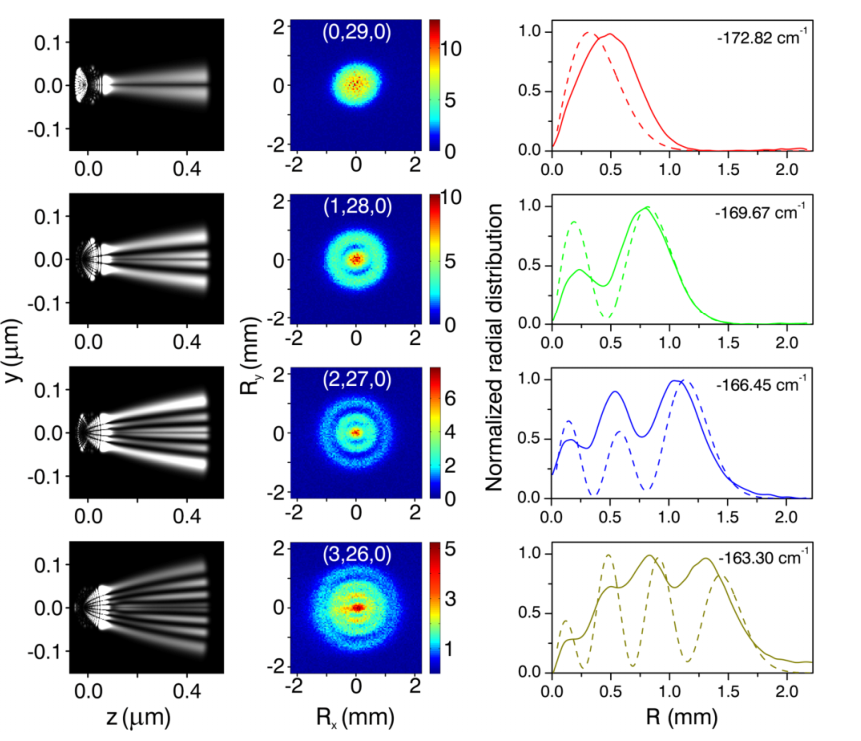
\includegraphics[height=0.8\textwidth]{figures/3.png}
    \end{figure}
\end{minipage}
\hfill
\begin{minipage}{0.35\textwidth}
    % \begin{figure}[h]
    %     \centering
    %     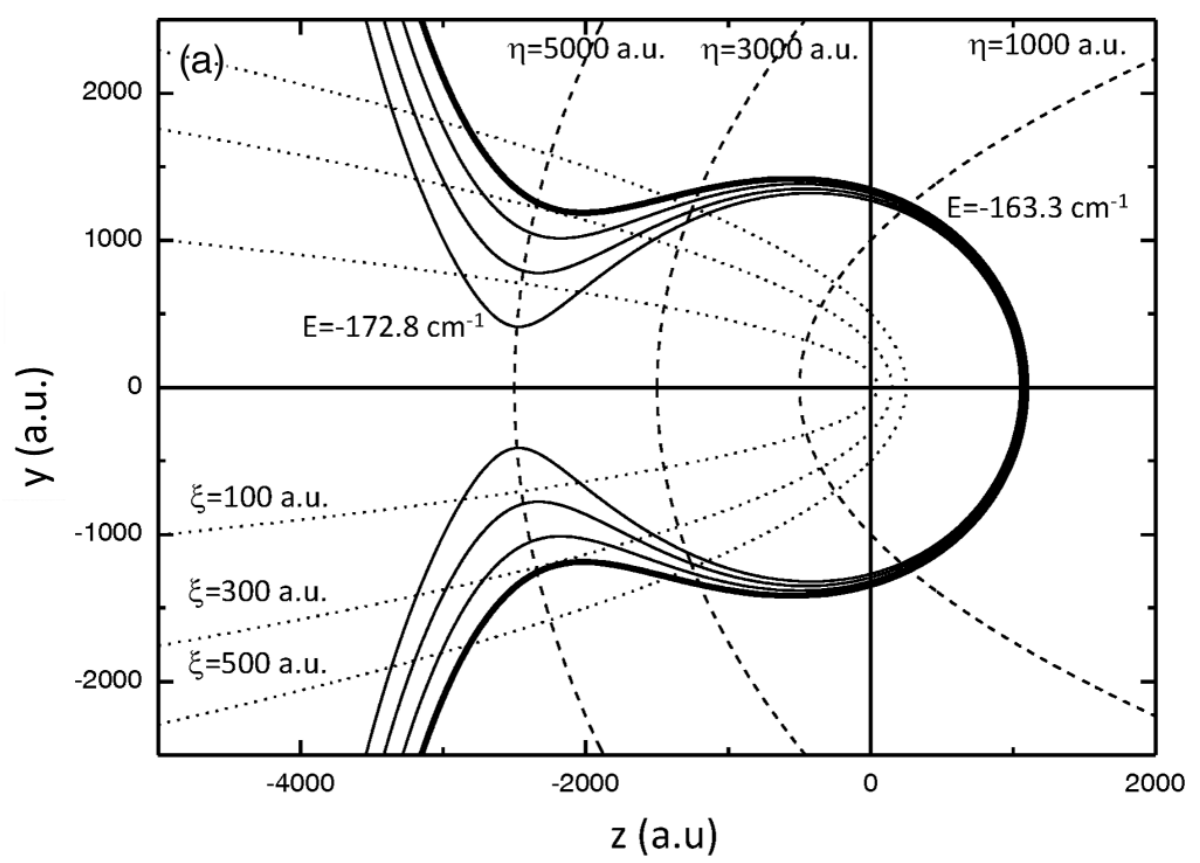
\includegraphics[width=1\textwidth]{figures/parabola.png}
    %     \caption{$n = n_1 + n_2 + |m| + 1$}
    %     %\label{fig:}
    % \end{figure}
        States $(n_1,n_2,m)$ 

        \cmark $m$ --- the magnetic quantum number. 

        \cmark $n_1, n_2$ --- related to the principal quantum number as\\
        $
            n = n_1 + n_2 + |m| + 1
        $
\end{minipage}


